\documentclass{article}

\usepackage{tikz}
\usetikzlibrary{automata, positioning, arrows}

\usepackage{amsthm}
\usepackage{amsfonts}
\usepackage{amsmath}
\usepackage{amssymb}
\usepackage{fullpage}
\usepackage{color}
\usepackage{parskip}
\usepackage{hyperref}
  \hypersetup{
    colorlinks = true,
    urlcolor   = blue,   % color of external links
    linkcolor  = blue,   % color of internal links
    citecolor  = blue,   % color of links to bibliography
    filecolor  = blue    % color of file links
  }

\usepackage{listings}

\definecolor{dkgreen}{rgb}{0,0.6,0}
\definecolor{gray}{rgb}{0.5,0.5,0.5}
\definecolor{mauve}{rgb}{0.58,0,0.82}

\lstset{frame=tb,
  language=Python, % change to any language you prefer
  aboveskip=3mm,
  belowskip=3mm,
  showstringspaces=false,
  columns=flexible,
  basicstyle={\small\ttfamily},
  numbers=none,
  numberstyle=\tiny\color{gray},
  keywordstyle=\color{blue},
  commentstyle=\color{dkgreen},
  stringstyle=\color{mauve},
  breaklines=true,
  breakatwhitespace=true,
  tabsize=3
}

% ---------------------------------------------------------------------
% Theorem/Definition/Remark Environments
% ---------------------------------------------------------------------
\newtheoremstyle{theorem}
  {\topsep}   % ABOVESPACE
  {\topsep}   % BELOWSPACE
  {\itshape\/}  % BODYFONT
  {0pt}       % INDENT (empty value is the same as 0pt)
  {\bfseries} % HEADFONT
  {.}         % HEADPUNCT
  {5pt plus 1pt minus 1pt} % HEADSPACE
  {}          % CUSTOM-HEAD-SPEC

\theoremstyle{theorem} 
   \newtheorem{theorem}{Theorem}[section]
   \newtheorem{corollary}[theorem]{Corollary}
   \newtheorem{lemma}[theorem]{Lemma}
   \newtheorem{proposition}[theorem]{Proposition}

\theoremstyle{definition}
   \newtheorem{definition}[theorem]{Definition}
   \newtheorem{example}[theorem]{Example}

\theoremstyle{remark}    
  \newtheorem{remark}[theorem]{Remark}

\setcounter{tocdepth}{3}    % This makes subsubsections appear in TOC
\setcounter{secnumdepth}{3} % This makes subsubsections numbered

% ---------------------------------------------------------------------
% Title and Author
% ---------------------------------------------------------------------
\title{DFAs and NFAs}
\author{Max Randall \\ Chapman University}
\date{\today}

% ---------------------------------------------------------------------
% BEGIN DOCUMENT
% ---------------------------------------------------------------------
\begin{document}

\maketitle

\setcounter{tocdepth}{3}
\tableofcontents

% ---------------------------------------------------------------------
% Introduction
% ---------------------------------------------------------------------
\section{Introduction}\label{sec:intro}
This week we covered ways to combine automata. We focused on the set theory used in the combination as well as some notation.
Lastly, we introduced Nondeterministic Finite Automatas, or NFAs.
\newpage
% ---------------------------------------------------------------------
% Week by Week (or Chapter by Chapter)
% ---------------------------------------------------------------------
\section{Exersizes}\label{sec:week-by-week}

\subsection{Extended Transition Functions}
\textbf{Brief summary of the question:}
Given the two DFAs below:
\begin{itemize}
  \item Compute the extended transition functions 
    \(\hat\delta^{(1)}(1,\,abaa)\) and \(\hat\delta^{(2)}(1,\,abba)\), 
    showing all steps.
  \item Describe the language accepted by each automaton.
\end{itemize}

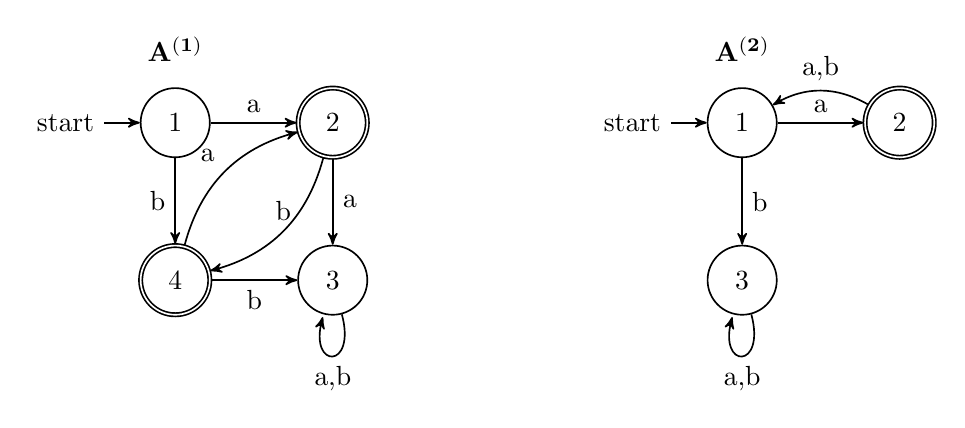
\begin{tikzpicture}[->, >=stealth', auto, node distance=2.0cm, semithick]
  % First automaton A^{(1)}
  \begin{scope}
    \node[state, initial] (1a) {1};
    \node[state, accepting, right of=1a] (2a) {2};
    \node[state, accepting, below of=1a] (4a) {4};
    \node[state, below of=2a] (3a) {3};

    \path (1a) edge              node {a} (2a)
               edge[left]       node {b} (4a)
          (2a) edge              node {a} (3a)
               edge[bend left,above]  node {b} (4a)
          (4a) edge[bend left]  node {a} (2a)
               edge[below]            node {b} (3a)
          (3a) edge[loop below] node {a,b} ();
    \draw node at (1a.north) [above=0.2cm] {\(\mathbf{A^{(1)}}\)};
  \end{scope}

  % Second automaton A^{(2)}
  \begin{scope}[xshift=7.2cm]
    \node[state, initial] (1b) {1};
    \node[state, accepting, right of=1b] (2b) {2};
    \node[state, below of=1b] (3b) {3};

    \path (1b) edge              node {a} (2b)
               edge              node {b} (3b)
          (2b) edge[bend right, above]  node {a,b} (1b)
          (3b) edge[loop below]  node {a,b} ();
    \draw node at (1b.north) [above=0.2cm] {\(\mathbf{A^{(2)}}\)};
  \end{scope}
\end{tikzpicture}

\textbf{1. Languages Accepted by Each Automaton}

\[
  L\bigl(A^{(1)}\bigr) \;=\;
    \bigl\{\,
      w \in \{a,b\}^+
      \;\mid\;
      \text{no two consecutive symbols in $w$ are the same}
    \bigr\}.
\]

\[
  L\bigl(A^{(2)}\bigr) \;=\;
    a\,(\,(\,a \mid b\,)\,a\,)^{*}
  \;=\;
  \bigl\{
    w \in \{a,b\}^*
    \;\mid\;
    w \text{ has odd length, starts with $a$, and every odd position is $a$}
  \bigr\}.
\]

\textbf{2. Extended Transition Functions}

\[
  \hat{\delta}^{(1)}\bigl(1,\;abaa\bigr) \;=\; 3
\]
\[
  \hat{\delta}^{(2)}\bigl(1,\;abba\bigr) \;=\; 3
\]

\bigskip

\subsection{Intersection Automaton \(\mathbf{A}\) for \(\mathbf{A^{(1)}}\) and \(\mathbf{A^{(2)}}\)}

We form the product (a.k.a.\ intersection) automaton 
\[
  A \;=\; 
  \bigl( Q^{(1)} \times Q^{(2)}, \;\Sigma,\;\delta,\;(q_0^{(1)},q_0^{(2)}),\;F^{(1)} \times F^{(2)}\bigr),
\]
where
\begin{itemize}
\item 
  \(Q^{(1)} = \{1,2,3,4\}\) with start state \(q_0^{(1)} = 1\) and final states \(F^{(1)} = \{2,4\}\),
\item 
  \(Q^{(2)} = \{1,2,3\}\) with start state \(q_0^{(2)} = 1\) and final states \(F^{(2)} = \{2\}\),
\item 
  \(\Sigma = \{a,b\},\)
\item 
  the transition function \(\delta\) on a pair \((p,q)\) and symbol \(x\in\{a,b\}\) is
  \[
    \delta\bigl((p,q),\,x\bigr)
    \;=\;
    \bigl(\delta^{(1)}(p,x),\;\delta^{(2)}(q,x)\bigr).
  \]
\item 
  the final (accepting) states are all pairs 
  \((p,q)\in Q^{(1)}\times Q^{(2)}\) with \(p\in F^{(1)}\) \emph{and} \(q\in F^{(2)}\).
\end{itemize}

\subsection*{Transition Diagram (Reachable Part)}
\textbf{Intersection Automaton Construction.}\\
Construct the intersection automaton \(A\) for \(A^{(1)}\) and \(A^{(2)}\) as given above 
by drawing its transition diagram. 
(If there are unreachable states, you do not have to draw them.)

Below is the transition diagram of \(A\), including only the reachable states from \(\bigl(1,1\bigr)\).  
Recall that the \emph{only} accepting pairs are those whose first coordinate is in \(\{2,4\}\) and second coordinate is \(2\). 
(Here we will see that \((4,2)\) is actually \emph{unreachable}, so \((2,2)\) is the only reachable accepting state.)

\begin{center}
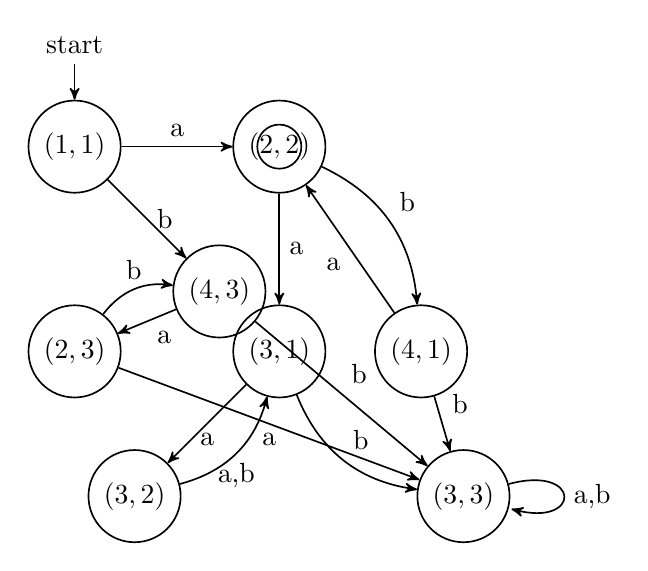
\begin{tikzpicture}[->, >=stealth', auto, node distance=2.6cm, semithick]

  % States
  \node[state,initial above] (11) {\((1,1)\)};
  \node[state] (22) [right of=11] {\((2,2)\)};
  \node[state] (43) [below right of=11] {\((4,3)\)};
  \node[state] (31) [below of=22] {\((3,1)\)};
  \node[state] (41) [below of=22, xshift=1.8cm] {\((4,1)\)};
  \node[state] (23) [below of=11] {\((2,3)\)};
  \node[state] (33) [below right of=31, xshift=0.5cm] {\((3,3)\)};
  \node[state] (32) [below left of=31] {\((3,2)\)};

  % Accepting
  \draw (22) circle [draw=black, very thick, x radius=0.28cm, y radius=0.28cm];

  % Transitions
  % (1,1)
  \path (11) edge node [above] {a} (22);
  \path (11) edge node [right] {b} (43);

  % (2,2)
  \path (22) edge node {a} (31);
  \path (22) edge [bend left] node {b} (41);

  % (4,3)
  \path (43) edge node {a} (23);
  \path (43) edge node {b} (33);

  % (3,1)
  \path (31) edge [below] node {a} (32);
  \path (31) edge [bend right] node {b} (33);

  % (4,1)
  \path (41) edge node {a} (22);
  \path (41) edge node {b} (33);

  % (2,3)
  \path (23) edge [below] node {a} (33);
  \path (23) edge [bend left, above] node {b} (43);

  % (3,3)
  \path (33) edge [loop right] node {a,b} (33);

  % (3,2)
  \path (32) edge [bend right, below] node {a,b} (31);

\end{tikzpicture}
\end{center}

\subsection*{Why \(L(A) = L(A^{(1)}) \cap L(A^{(2)})\)?}

By construction, \(A\) simulates both \(A^{(1)}\) and \(A^{(2)}\) in parallel:
\begin{itemize}
\item 
  Starting in \(\bigl(q_0^{(1)},q_0^{(2)}\bigr)\), 
  reading each symbol \(x\in\{a,b\}\) goes to 
  \(\bigl(\delta^{(1)}(p,x),\,\delta^{(2)}(q,x)\bigr)\).
\item 
  A string \(w\) is accepted by \(A\) if and only if, after reading \(w\), 
  the first coordinate is in \(F^{(1)}\) \emph{and} 
  the second coordinate is in \(F^{(2)}\). 
\end{itemize}
Hence a string is accepted precisely when \emph{both} \(A^{(1)}\) and \(A^{(2)}\) accept it. 
Thus \(L(A)=L(A^{(1)})\cap L(A^{(2)})\).

\subsection*{Changing \(\mathbf{A}\) to Obtain Union}

If we want \emph{union} rather than intersection, we can keep the same set of states, start state, and transitions, but change the accepting condition so that a pair \((p,q)\) is final whenever \emph{either} \(p\in F^{(1)}\) \textbf{or} \(q\in F^{(2)}\).  
Concretely,
\[
  F' \;=\; 
    \bigl(F^{(1)}\times Q^{(2)}\bigr) 
    \;\cup\; 
    \bigl(Q^{(1)}\times F^{(2)}\bigr).
\]
Then the resulting DFA \(A' = (Q,\Sigma,\delta,(q_0^{(1)},q_0^{(2)}),F')\) accepts 
\[
  L(A') = L(A^{(1)}) \;\cup\; L(A^{(2)}).
\]

\newpage

\subsection{Exercise 2.2.7}
\noindent
\textbf{Claim.} Let \(A\) be a DFA, and let \(q\) be a particular state of \(A\) such that 
\(\delta(q,a) = q\) for \textit{every} input symbol \(a\) in the alphabet.  
Then for any input string \(w\), we have \(\delta(q,w) = q\).

\bigskip
\noindent
\textbf{Proof (by induction on the length of \(w\)):}

\begin{itemize}
\item \textbf{Base Case:}  
  If \(\lvert w\rvert = 0\), then \(w = \varepsilon\).  
  By definition of the extended transition function, 
  \(\delta(q,\varepsilon) = q\).  
  Hence the statement holds for all strings of length 0.

\item \textbf{Inductive Step:}  
  Suppose the statement holds for all strings of length \(n\).  
  Let \(w\) be any string of length \(n+1\).  
  We can write \(w = x\,a\), where \(\lvert x\rvert = n\) and \(a\) is a single input symbol.  
  By the definition of the extended transition function,
  \[
    \delta(q,w) \;=\; \delta\bigl(q,\;x\,a\bigr) 
                   \;=\; \delta\bigl(\delta(q,x),\,a\bigr).
  \]
  By the inductive hypothesis, \(\delta(q,x) = q\).  
  Therefore
  \[
    \delta\bigl(\delta(q,x),\,a\bigr) 
    \;=\; \delta(q,a) 
    \;=\; q,
  \]
  because \(\delta(q,a) = q\) for every input symbol \(a\) by assumption.
\end{itemize}

\noindent
Thus, by mathematical induction, \(\delta(q,w) = q\) for every string \(w\in\Sigma^*\). 
\qedsymbol

\section{Chapter 2.3}

The text introduces the \emph{extended transition function} \(\hat{\delta}\) for an NFA. 
Recall that \(\delta\) itself only covers a single state and input symbol, while 
\(\hat{\delta}\) handles a state (or set of states) and an entire string. We define 
\(\hat{\delta}\) by the rules:

\begin{itemize}
\item
  \(\hat{\delta}(q,\varepsilon) = \{\,q\}\). 
  (If we consume no input, we remain in the same state.)
\item
  \(\hat{\delta}(q,\,xa) \;=\;\bigcup_{\,p \,\in\, \hat{\delta}(q,\,x)\!}\,\delta(p,\,a)\). 
  (If \(w=xa\), first move on \(x\), then from each possible state, move on symbol \(a\).)
\end{itemize}

This captures \textbf{nondeterminism} because we allow multiple possible next states. An NFA 
\emph{accepts} a string \(w\) if at least one of the states in \(\hat{\delta}(q_{0}, w)\) is 
in the set of accepting states. Several examples illustrate the step-by-step use of 
\(\hat{\delta}\), showing that an NFA may branch along several paths of computation.

\paragraph{Subset Construction.}
We can convert any NFA \(N\) into a DFA \(D\) recognizing the same language by 
the \emph{subset construction}, in which each subset of \(N\)'s states becomes a single 
state in \(D\). Concretely:
\begin{itemize}
\item
  The states of \(D\) are all subsets of \(N\)'s state set.
\item
  \(D\)'s start state is the subset \(\{\,q_{0}\}\) containing only the NFA's start state.
\item
  A subset \(S\) of \(N\)'s states is \emph{accepting} in \(D\) if \(S\) contains at least 
  one of \(N\)'s accepting states.
\item
  For each subset \(S\subseteq Q\) and each symbol \(a\in\Sigma\),
  \[
    \delta_{D}(S,a)
    \;=\;
    \bigcup_{p\in S}\,\delta_{N}(p,a).
  \]
\end{itemize}
This process ensures \(L(D)=L(N)\). Although the subset construction can produce a worst-case 
exponential blowup in the number of states, in practice it often yields fewer states than 
the worst‐case bound. Thus, we see every language recognized by an NFA also has a DFA 
recognizer, proving the equivalence of NFAs and DFAs. 

\newpage

\noindent
\section{Conclusion} \\
Throughout these problems and readings, we have deepened our understanding of both deterministic 
and nondeterministic finite automata. We explored extended transition functions, which formalize 
how automata process entire strings. We examined the product automaton construction, which 
combines two DFAs for intersection. We also saw that modifying acceptance states can yield union. 
Through the subset construction, we established the equivalence of NFAs and DFAs: any NFA can be 
systematically converted into a DFA that accepts the same language. Consequently, these powerful 
concepts and proofs underscore the robustness of finite automata theory, vital across both theory 
and practice, and widely used today.

\textbf{ Interesting question: Maximal Blow-Up in the Subset Construction.}\\
    Can you describe a concrete NFA of \(n\) states that forces its equivalent DFA 
    (from the subset construction) to use all \(2^n\) possible subsets as distinct states? 
    Moreover, how can we prove that no smaller DFA can recognize the same language?

\newpage

\begin{thebibliography}{99}

    \bibitem[HMU] 
    J.~E.~Hopcroft, R.~Motwani, J.~D.~Ullman: 
    \emph{Introduction to Automata Theory, Languages, and Computation (3rd Edition)}, 
    \href{https://archive.org/details/hopcroft-motwani-ullman-introduction-to-automata-theory-languages-and-computations-3rd-edition/page/65/mode/1up?view=theater}{Archive.org Link}.
    
\end{thebibliography}    

\end{document}
